\documentclass[20pt]{beamer}

\usetheme{Berkeley}
\setbeamertemplate{caption}[numbered]
\everymath=\expandafter{\the\everymath\displaystyle}

\ifdefined\pdftexversion\else  % non-pdftex case.
	\usepackage{fontspec}
\fi
\makeatletter\@ifpackageloaded{underscore}{}{\usepackage[strings]{underscore}}\makeatother

\newcommand{\diff}[1]{\operatorname{d}#1}
\renewcommand{\vec}[1]{\boldsymbol{#1}}


\author{Henry Ding}
\date{\today}
\title{Lesson 5: Applications of Newton's Laws}


\begin{document}

\frame{\titlepage}

\section{Vector Notation Conventions}

\begin{frame}
	\frametitle{Vector Notation Conventions}
	When labeling forces, accelerations, etc. on free body diagrams, the symbol next to a force often represents the vector's magnitude.

	A non-bold letter often represents a vector's magnitude. For example, the magnitude of force $\vec{F}$ can be written as $F$.
	\begin{figure}[ht]
		\centering
		\inkfig{0.8\textwidth}{vectornotation}
		%\caption{}
		\label{fig:vectornottation}
	\end{figure}
\end{frame}


\section{Tension}

\begin{frame}
	\frametitle{Thin Strings}
	\begin{definition}
		Tension always points along a \textbf{thin string}.
	\end{definition}
	\begin{figure}[ht]
		\centering
		\inkfig{\textwidth}{thinstring}
		\caption{}
		%\label{fig:thinstring}
	\end{figure}
\end{frame}

\begin{frame}
	\frametitle{Massless Strings}
	\begin{definition}
		The \textit{magnitude} of tension is constant throughout a \textbf{massless string}.
	\end{definition}
	\begin{figure}[ht]
		\centering
		\inkfig{0.7\textwidth}{masslessstring}
		%\caption{}
		\label{fig:masslessstring}
	\end{figure}
	\begin{theorem}
		Along the direction of the string,
		\begin{align*}
			F_\mathrm{net} = T_R - T_L = ma,
		\end{align*}
		but $m = 0$ so $T_R = T_L$. The tension is constant throughout the string.
	\end{theorem}
	\begin{alertblock}{Massless String Approximation} % TODO: introduce approximations in physics during the air resistance discussion
		Real strings are not massless! However, we can approximately ignore a string's mass if it's mass is small compared to the mass of other objects.
	\end{alertblock}
\end{frame}

\begin{frame}
	\frametitle{Inextensible String}
	\begin{definition}
		An \textbf{inextensible string} has constant length.
	\end{definition}
	\begin{example}
		\begin{figure}[ht]
			\centering
			\inkfig{\textwidth}{inextensiblestring}
			%\caption{}
			\label{fig:inextensiblestring}
		\end{figure}
	\end{example}
\end{frame}

\begin{frame}
	\frametitle{Massless String Example}
	\begin{example}
		Arthur pulls a massless string with a force $\vec{P}$. The string is connected to a crate with mass $m$. Find the crate's acceleration.
		\begin{figure}[ht]
			\centering
			\inkfig{\textwidth}{crate1}
			%\caption{}
			\label{fig:crate1}
		\end{figure}
	\end{example}
\end{frame}

\begin{frame}
	\frametitle{Solving Force Problems}
	\begin{block}{Identify Forces}
		Arthur's pulling force, and tension in the string
	\end{block}
	\begin{block}{Draw Free Body Diagrams}
		You may need to apply Newton's Third Law.
		\begin{figure}[ht]
			\centering
			\inkfig{0.8\textwidth}{crate1-fbd}
			%\caption{}
			\label{fig:crate1-fbd}
		\end{figure}
	\end{block}
	\begin{block}{Write Newton's Second Law and Solv and Solve}
		Recall
		\begin{align*}
			\vec{F}_\mathrm{net} = m \vec{a}.
		\end{align*}
		For the massless string, $T = P$. For the crate,
		\begin{align*}
			P = ma \Rightarrow a = P / m.
		\end{align*}
	\end{block}
\end{frame}

\begin{frame}
	\frametitle{Another Massless String Example}
	\begin{example}
		Clinton pulls on a massless string with a force $\vec{P}$. The string is connected to a crate of mass $m_1$, which is connected to another crate of mass $m_2$ via a second massless string. Find the tension in the string between both crates. What is the acceleration of each create?
		\begin{figure}[ht]
			\centering
			\inkfig{0.8\textwidth}{crate2}
			%\caption{}
			\label{fig:crate2}
		\end{figure}
	\end{example}
\end{frame}

\begin{frame}
	\frametitle{Elevator Example}
	\begin{example}
		A string connects a mass $m$ to the roof of an elevator. What is the tension in the string when the elevator rises at a constant velocity? What is the tension when the elevator accelerates downwards with magnitude $a$?
		\begin{figure}[ht]
			\centering
			\inkfig{\textwidth}{elevator1}
			%\caption{}
			\label{fig:elevator1}
		\end{figure}
	\end{example}
\end{frame}

\begin{frame}
	\frametitle{Atwood Machines}
	Atwood machines feature in many problems and consist of masses connected to strings and pulleys. Remember strings are inextensible!
	\begin{example}
		Blocks of mass $m_1$ and $m_2$ are connected to the left/right of a pulley. Find the tension in the string and the blocks' accelerations.
		\begin{figure}[ht]
			\centering
			\inkfig{0.3\textwidth}{atwood1}
			%\caption{}
			\label{fig:atwood1}
		\end{figure}
	\end{example}
\end{frame}

\section{Friction}

\begin{frame}
	\frametitle{Static and Kinetic Friction}
	Consider pushing a block with a growing force $P$. At first, the block stays still due to friction. When $P$ is large enough, $P$ will overcome friction and the block will accelerate.
	\begin{figure}[ht]
		\centering
		\inkfig{0.8\textwidth}{statickinetic}
		%\caption{}
		\label{fig:statickinetic}
	\end{figure}
	\begin{figure}[ht]
		\centering
		\mplfig{frictiongraph.pgf}
		%\caption{}
		\label{fig:frictiongraph}
	\end{figure}
\end{frame}

\begin{frame}
	\frametitle{Laws of Friction}
	\begin{theorem}
		Static friction has a maximum magnitude of
		\begin{align*}
			\vec{f}_s \leq \mu_s \vec{N}.
		\end{align*}
		Kinetic friction always has a magnitude of
		\begin{align*}
			\vec{f}_k = \mu_k N.
		\end{align*}
	\end{theorem}
	\begin{theorem}
		Kinetic friction must be smaller than or equal to the maximum static friction, so $\mu_s \geq \mu_k$.
	\end{theorem}
\end{frame}

\begin{frame}
	\frametitle{Microscopic Basis of Friction}
	In the real world, surfaces are not smooth but contain microscopic bumps.
	When two surfaces are pushed together, the surface bumps ``cold weld'' together and stick.
	If the surfaces move relative to each other, the welds resist the movement before break apart, causing friction.
	Greater normal force $N$ cases more welds to form, leading to higher friction force.
	\begin{figure}[ht]
		\centering
		\inkfig{0.6\textwidth}{microscopicfriction}
		%\caption{}
		\label{fig:microscopicfriction}
	\end{figure}
\end{frame}

\begin{frame}
	\frametitle{Horse Riddle}
	\begin{example}
		A farmer hitches the lazy horse Agnes to a wagon. Remembering Newton's Third Law, Agnes claims that for any she force pulls the wagon, the wagon will pull her back with the same force. Pulling the wagon is therefore futile, and the farmer should just give her some grass to eat (yum). What's wrong with this argument?
	\end{example}
\end{frame}

\begin{frame}
	\frametitle{Atwood Machine Example}
	\begin{example}
		A mass $m_1$ lies on a horizontal surface with coefficients of friction $\mu_s = \mu_k = \mu$. The mass $m_1$ is connected by a string hung over a pulley to a vertically hanging mass $m_2$. Find the blocks' accelerations.
		\begin{figure}[ht]
			\centering
			\inkfig{0.7\textwidth}{atwood2}
			%\caption{}
			\label{fig:atwood2}
		\end{figure}
	\end{example}
\end{frame}

\section{Inclined Planes}

\begin{frame}
	\frametitle{Inclined Planes}
	\begin{definition}
		An \textbf{inclined plane} is a ramp.
	\end{definition}
	Remember, the orientation of a coordinate system can be changed for convenience.
	\begin{figure}[ht]
		\centering
		\inkfig{\textwidth}{planeaxes}
		%\caption{}
		\label{fig:planeaxes}
	\end{figure}
\end{frame}

\begin{frame}
	\frametitle{Inclined Plane Example}
	\begin{example}
		A mass lies on an inclined plane at an angle $\theta$ to the horizontal. A string parallel to the incline holds the mass in place. Find the tension in the string and the normal force on the block. If the string is cut, what is the block's acceleration?
	\end{example}
\end{frame}

\begin{frame}
	\frametitle{Another Inclined Plane Example}
	\begin{example}
		A block lies on an inclined plane at an angle $\theta$ to the horizontal. $\theta$ is slowly increased from $0$. The block remains at rest on the incline until $\theta$ reaches a maximum angle $\theta_m$, when the block slips. What is the coefficient of static friction between the block and the incline?
	\end{example}
\end{frame}

\begin{frame}
	\frametitle{Uniform Circular Motion Example}
	\begin{example}
		A mass $m$ is connected to the ceiling by a string of $L$. The mass travels in a horizontal circle at constant speed while the string makes an angle $\theta$ to the vertical. Find the period of revolution.
		\begin{figure}[ht]
			\centering
			\inkfig{0.4\textwidth}{conicalpendulum}
			%\caption{}
			\label{fig:conicalpendulum}
		\end{figure}
	\end{example}
\end{frame}

\begin{frame}
	\frametitle{Another Uniform Circular Motion Example}
	\begin{example}
		An electric car of mass $m$ drives along a circular track of radius $R$. Find the minimum coefficient of friction required for the car to travel at a constant speed $v$.
	\end{example}
\end{frame}

\section{Springs}

\begin{frame}
	\frametitle{Springs}
	% TODO : figure out if I need to talk about SHM here
	\begin{theorem}{Hooke's Law}
		A massless spring is stretched $\Delta x$ beyond its rest length. Then, the force exerted on its ends has magnitude
		\begin{align*}
			F_s = -k \Delta x.
		\end{align*}
	\end{theorem}
\end{frame}

\section{Homework 5}

\begin{frame}
	\frametitle{Homework 5}
	\begin{block}{Textbook Problems}
		\begin{itemize}
			\item \href{https://openstax.org/books/physics/pages/5-problems}{OpenStax Physics (High School) Chapter 5 Problems} 31, 32
		\end{itemize}
	\end{block}
\end{frame}

\begin{frame}
	\frametitle{Homework 5}
	\begin{block}{\href{https://www.wiley.com/en-us/Physics\%2C+Volume+1\%2C+5th+Edition-p-9780471320579}{\textit{Physics}, Volume 1, 5th Edition, Chapter 5 Multiple Choice 3}}
		A wooden box is sitting on a table. The normal force on the box from the table is $\SI{75}{\newton}$. A second identical box is placed on top of the first box. The normal force on the first box by the table will
		\begin{enumerate}
			\item[(A)] decrease.
			\item[(B)] remain at $\SI{75}{\newton}$.
			\item[(C)] increase to $\SI{150}{\newton}$.
			\item[(D)] increase to $\SI{300}{\newton}$.
		\end{enumerate}
	\end{block}
	\begin{block}{\textit{Physics}, Volume 1, 5th Edition, Chapter 5 Multiple Choice 7}
		Which statement is correct about the weight (another name for gravity force) of an object and the force of kinetic friction on that object?
		\begin{enumerate}
			\item[(A)] The weight is always greater than the frictional force.
			\item[(B)] The weight is always equal to the frictional force.
			\item[(C)] The weight is less than the frictional force for sufficiently light objects.
			\item[(D)] The weight can be more or less than the frictional force.
		\end{enumerate}
	\end{block}
\end{frame}

\begin{frame}
	\frametitle{Homework 5}
	\begin{block}{\textit{Physics}, Volume 1, 5th Edition, Chapter 5 Exercise 2 (modified)}
		An elevator weighing $\SI{500}{\kilogram}$ is pulled upward by a cable with an acceleration of $\SI{3.8}{\meter/\second^2}$. What is the tension in the cable? What is the tension when the elevator is accelerating downard at $\SI{3.8}{\meter/\second^2}$ but still moving upward?
	\end{block}
\end{frame}

\begin{frame}
	\frametitle{Homework 5}
	\begin{block}{\textit{Physics}, Volume 1, 5th Edition, Chapter 5 Exercise 13}
		A horizontal bar is used to support a $\SI{75}{\kilogram}$ object between two walls, as shown below. The equal forces $F$ exerted by the bar against the walls can be varied by adjusting the length of the bar. Only friction between the ends of the bar and the walls supports the system. The coefficient of static friction between bar and walls is $0.41$. Find the minimum value of the forces $F$ for the system to remain at rest.
		\begin{figure}[ht]
			\centering
			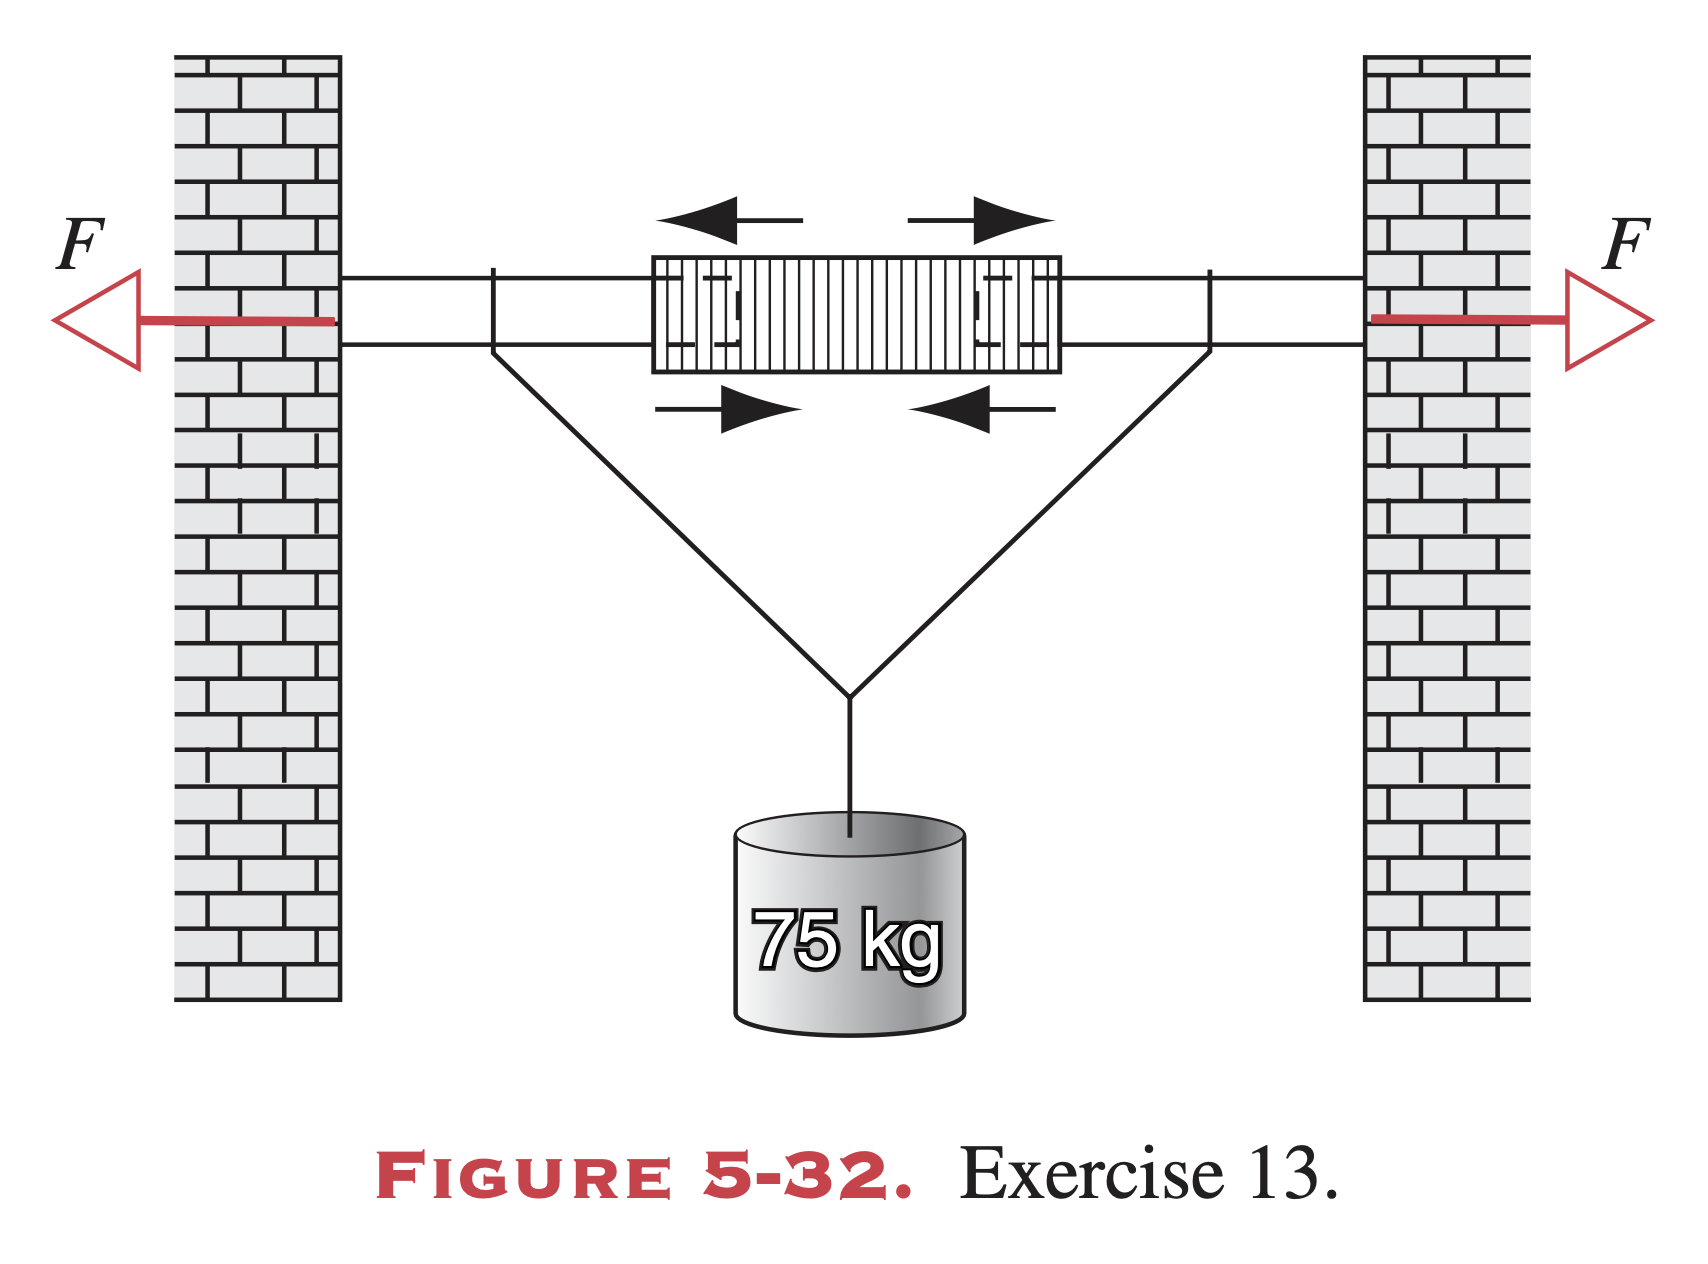
\includegraphics[width=0.5\textwidth]{HRKc5e13.png}
			%\caption{}
			\label{fig:HRKc5e13}
		\end{figure}
	\end{block}
\end{frame}

\begin{frame}
	\frametitle{Homework 5}
	\begin{block}{\textit{Physics}, Volume 1, 5th Edition, Chapter 5 Exercise 28}
		Block $m_1$ in in the figure below has a mass of $\SI{4.20}{\kilogram}$ and block $m_2$ has a mass of $\SI{2.30}{\kilogram}$. The coefficient of kinetic friction between $m_2$ and the horizontal plane is $0.47$. The inclined plane is frictionless. Find (a) the acceleration of the blocks and (b) the tension in the string.
		\begin{figure}[ht]
			\centering
			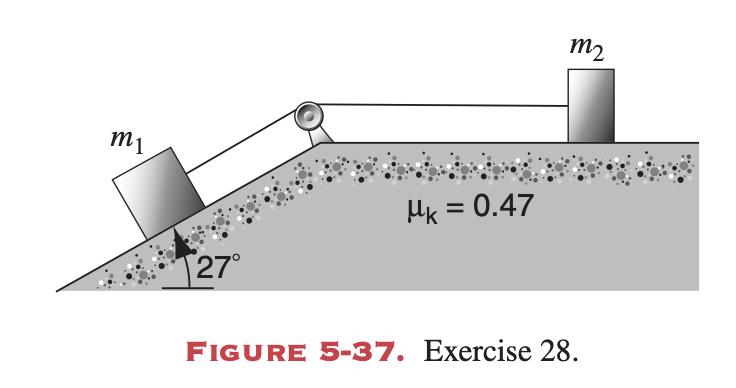
\includegraphics[width=0.5\textwidth]{HRKc5e28.png}
			%\caption{}
			\label{fig:HRKc5e28}
		\end{figure}
	\end{block}
\end{frame}

\begin{frame}
	\frametitle{Homework 5}
	\begin{block}{\textit{Physics}, Volume 1, 5th Edition, Chapter 5 Exercise 39}
		A disk of mass $m$ on a frictionless table is attached to a hanging cylinder of mass $M$ by a cord through a hole in the table. Find the speed with which the disk must move in a circle of radius $r$ for the cylinder to stay at rest.
		\begin{figure}[ht]
			\centering
			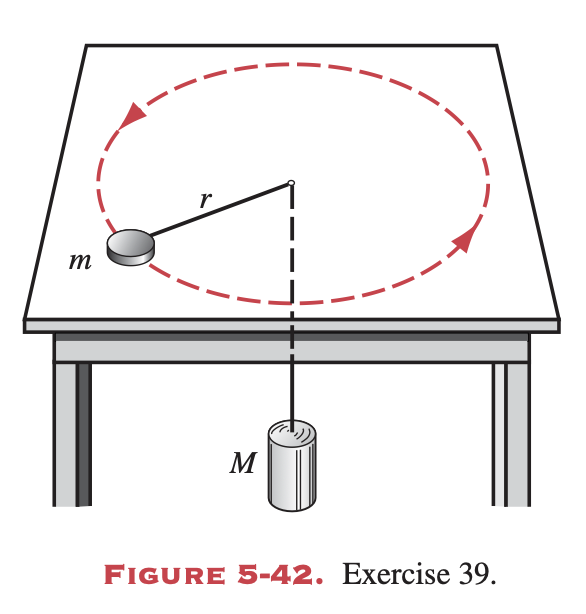
\includegraphics[width=0.5\textwidth]{HRKc5e39.png}
			%\caption{}
			\label{fig:HRKc5e39}
		\end{figure}
	\end{block}
\end{frame}


\end{document}
